\documentclass[11pt]{article}   % tipo de documento e tamanho das letras

% os seguintes pacotes estendem a funcionalidade básica:
\usepackage[a4paper, total={16cm, 24cm}]{geometry} % tamanho da pagina e do texto
\usepackage[portuguese]{babel}  % traduz para portugues
\usepackage[utf8]{inputenc}
\usepackage{graphicx}           % graficos
\usepackage{amsmath}            % matematica
\usepackage{tikz}               % diagramas
    \usetikzlibrary{shadows}
\usepackage{booktabs}           % tabelas com  melhor aspecto
\usepackage[colorlinks=true]{hyperref}           % links para partes do documento ou para a web
\usepackage{listings}           % incluir codigo
    \renewcommand\lstlistingname{Listagem}  % Listing em portugues
    \lstset{numbers=left, numberstyle=\tiny, numbersep=5pt, basicstyle=\footnotesize\ttfamily, frame=tb,rulesepcolor=\color{gray}, breaklines=true}
\usepackage{blindtext}

% -------------------------------------------------------------------------------------------
\title
{
    
\includegraphics[width=0.3\textwidth]{images/logo_universidade.png}
    \\[0.1cm]
    \textbf{Códigos Ambíguos} \\
    Programação III
}

\author
{
    \textbf{Professores:} Salvador Abreu \\ Pedro Patinho \\
    \textbf{Realizado por:} Miguel de Carvalho (43108) \\ João Pereira (42864) 
}
\date{\today}

% -------------------------------------------------------------------------------------------
%                                Body                                                       %
% -------------------------------------------------------------------------------------------

\begin{document}
\maketitle

% -------------------------------------------------------------------------------------------
\section{Introdução} 
\hspace{0,5cm}Neste trabalho foi solicitado a realização de um programa que encontre 
\textbf{Palavras Ambíguas} numa gramática binária, como representado na figura abaixo.

\begin{figure}[h!]
    \begin{center}
        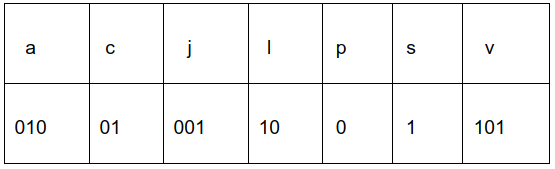
\includegraphics[width=0.5\textwidth]{images/gramatica.png}
        \caption{Exemplo de uma gramática binária}
    \end{center}
\end{figure}

No exemplo acima, a palavra \textbf{c} é ambígua com a palavra \textbf{ps}, pois ambas as
palavras correspondem ao mesmo código binário (\textbf{01}).
Outro exemplo de \textbf{palavras ambíguas} é entre a palavra \textbf{l} e a palavra \textbf{sp},
pois ambas as palavras correspondem ao mesmo código binário \textbf{10}.

No nosso programa deverá mostrar unicamente as \textbf{Palavras Ambíguas} que apresentam uma
\textbf{menor} ordem \textbf{lexicográfica}.
% -------------------------------------------------------------------------------------------
\section{Implementação}

\hspace{0,5cm}Inicialmente pensámos como deveríamos proceder para realizar o trabalho, ou seja,
começámos por fazer o "pensamento" em papel. 

De seguida na nossa primeira tentativa começamos por implementar tudo em \textbf{Prolog}, mas 
chegamos à conclusão de que o nosso pensamento não era o mais eficaz. Pois, gerávamos todas as
palavras possíveis e de seguida fazíamos comparações entre si.

Por conseguinte começámos por fazer esta implementação na linguagem \textbf{OCaml}, pois esta
linguagem permite-nos fazer as condições de uma maneira que é mais familiar às outras linguagens.
% -------------------------------------------------------------------------------------------
\newpage
\section{Funções}

\subsection{Funções Auxiliares}

\begin{itemize}
    \item \verb|getWord| - recebe um \textbf{tuplo} e devolve a 2ª posição (\textbf{word});
    \item \verb|getBin| - recebe um \textbf{tuplo} e devolve a 1ª posição (\textbf{binário});
    \item \verb|convert| - recebe um \textbf{tuplo} em que a 1ª posição é um \textbf{char} e 
    converte essa 1ª posição do \textbf{tuplo} em uma \textbf{lista} que contem uma \textbf{string}
    e devolve esse \textbf{tuplo} modificado;
    \item \verb|convertList| - recebe uma \textbf{lista} de \textbf{tuplos} e utiliza o \verb|convert|
    em cada um dos seus \textbf{tuplos} e devolve essa \textbf{lista} convertida;
    \item \verb|printWord| - recebe uma \textbf{lista} de \textbf{strings} (\textbf{words}) e 
    \textit{printa} usando a função \verb|print_string|;
    \item \verb|printBin| - recebe uma \textbf{lista} de \textbf{inteiros} (\textbf{bins}) e 
    \textit{printa} usando a função \verb|print_int|;
    \item \verb|printWordList| - recebe uma \textbf{lista} de \textbf{tuplos} e \textit{printa} só a 
    \textbf{words} usando a função \verb|getWord| e \verb|printWord|;
    \item \verb|printBinList| - recebe uma \textbf{lista} de \textbf{tuplos} e \textit{printa} só as 
    \textbf{bins} usando a função \textit{getBin} e \textit{printBin};
    \item \verb|printCodeList| - recebe uma \verb|lista| de \verb|tuplos| e \textit{printa} o conteúdo
    utilizando o \verb|printWordList| e \verb|printBinList|;
    \item \verb|merge| - recebe dois \textbf{tuplos} cada um com a \textbf{word} e o respetivo \textbf{bin}
    e faz \textit{append} (\verb|@|) devolvendo um único \textbf{tuplo} com a junção das \textbf{words} e 
    do respetivo \textbf{bin};
    \item \verb|listHeader| - recebe uma \textbf{lista} e devolve o \textbf{topo} dessa \textbf{lista};
    \item \verb|result| - recebe uma \textbf{lista} e devolve um \textbf{tuplo} com o \textbf{código binário}
    e as respetivas palavras ambíguas;
    \item \verb|print_result| - recebe um \textbf{tuplo} e \textit{printa} as \textbf{palavras ambíguas} com
    o respetivo \textbf{código binário} com um formato específico.
\end{itemize}

\subsection{Funções Principais}

\begin{itemize}
    \item \verb|main| - recebe uma \textbf{lista} de \textbf{tuplos convertidos} pela função 
    \verb|convertList| e devolve o resultado que são as 2 \textbf{palavras ambíguas} e o respetivo 
    \textbf{código binário};
    \item \verb|is_ambigous| - recebe uma \textbf{lista} de \textbf{tuplos} e verifica se os 
    \textbf{bins} dessa \textbf{lista} correspondem a mais do que uma \textbf{word} utilizando 
    a função \verb|process|. Caso não seja, retorna uma \textbf{lista vazia}, caso contrário, 
    devolve a resposta da \textbf{ambiguidade};
    \item \verb|process| - recebe uma \textbf{lista} de \textbf{tuplos} e um determinado 
    \textbf{tuplo} dessa lista, para cada membro dessa lista vai verificar se o \textbf{bin}
    é igual e a \textbf{word} é diferente da que está a ser processada, caso isto aconteça
    estamos perante uma \textbf{palavra ambígua}. Caso isto não aconteça o \verb|process|
    retorna uma \textbf{lista} vazia.
    A \textbf{palavra ambígua} devolvida vai ser a primeira encontrada ou a que apresenta
    menor \textbf{word} ou a menor \textbf{bin} do que a que já tinha sido encontrada inicialmente;
    \item \verb|loop_append| - recebe uma \textbf{lista} de \textbf{tuplos} e um determinado
    \textbf{tuplo} e devolve uma \textbf{lista} com as combinações das \textbf{words};
    Por exemplo, recebe \verb|[('a',01),('b', 101), ('c', 0)]| e \verb|('a')| e devolve 
    \verb|[('aa', 0101), ('ab', 01101), ('ac', 010)]|;
    \item \verb|loop_merge| - recebe uma \textbf{lista convertida} e uma \textbf{lista vazia}, essa
    \textbf{lista vazia} vai ser preenchida com os resultados da função \verb|loop_append|;
    \item \verb|list_merge| - recebe duas \textbf{listas} e retorna uma \textbf{lista} com o 
    conteúdo das duas \textbf{listas} sem existir repetição.
\end{itemize}
% -------------------------------------------------------------------------------------------
\section{Dificuldades sentidas}

Durante a elaboração do trabalho sentimos dificuldades na manipulação das \textbf{listas} e
adaptar o nosso pensamento a \textbf{linguagens} com um pensamento \textbf{recursivo}.
% -------------------------------------------------------------------------------------------
\section{Conclusão} % Conclusão
\hspace{0,5cm}Em suma, com a realização deste trabalho "Códigos Ambíguos" ficámos muito mais 
esclarecidos sobre o funcionamento de um programa que encontre os mesmos. \par
Saliento também que nos ajudou a perceber melhor como funcionam as linguagens \textbf{declarativas},
como \textbf{Prolog} e \textbf{OCaml}.
% -------------------------------------------------------------------------------------------
\end{document}